\documentclass[12pt]{beamer}
\usetheme{Madrid}
\usepackage[utf8]{inputenc}
\usepackage{amsmath}
\usepackage{amsfonts}
\usepackage{amssymb}
\usepackage{graphicx}
\usepackage{caption}
\usepackage{subcaption}
\setcounter{tocdepth}{4}
\setcounter{secnumdepth}{4}
\title{Convolutional Neural Networks}
%\setbeamercovered{transparent} 
%\setbeamertemplate{navigation symbols}{} 
%\logo{} 
%\institute{} 
%\date{} 
%\subject{} 

\author{
\linebreak
Julius Taylor \\ \texttt{0000000} \\ \href{mailto:stud3@email.com}{stud3@email.com}
 \and   
 \linebreak
Shawn Cala \\ \texttt{4921431} \\ \href{mailto:shawn.cala@gmail.com}{shawn.cala@gmail.com}
}

\begin{document}

\begin{frame}
\titlepage
\end{frame}
\frame{\frametitle{Table of Contents}\tableofcontents} 
%\begin{frame}
%\tableofcontents
%\end{frame}
\section{Background and Motivation}
\subsection{Background and Motivation - Neural Networks}
\begin{frame}{Background and Motivation - Neural Networks}

Primary motivation: Neural Networks mathematically simulate biological functionalities of the human brain
\begin{figure}
\begin{subfigure}{.5\textwidth}
  \centering
  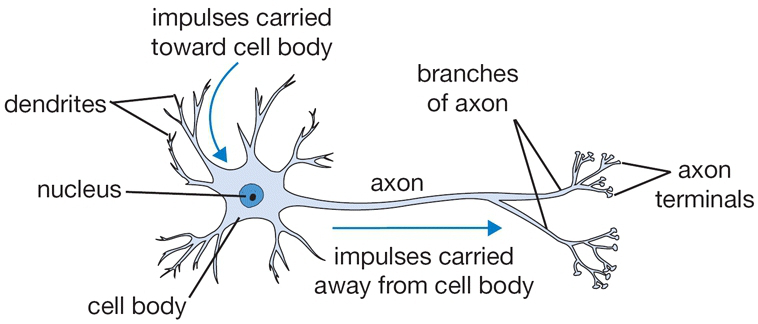
\includegraphics[width=\linewidth,height=0.35\textheight]{images/neuron.png}
  \caption{biological model}
  \label{fig:sub1}
\end{subfigure}%
\begin{subfigure}{.5\textwidth}
  \centering
  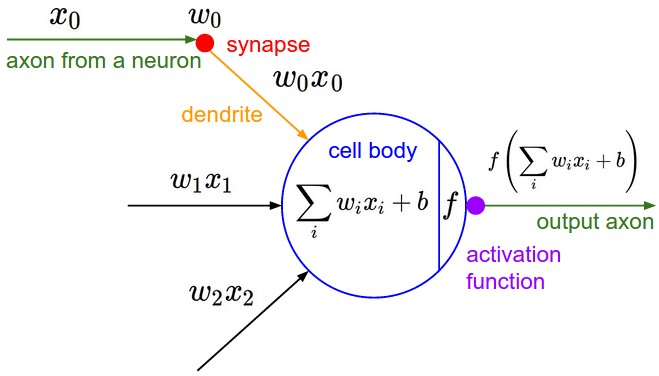
\includegraphics[width=\linewidth,height=0.35\textheight]{images/neuron_model.jpeg}
  \caption{mathematical representation}
  \label{fig:sub2}
\end{subfigure}
\caption{neuronal model and computational abstraction}
\label{fig:abstract}
\end{figure}

\end{frame}
\subsection{Background and Motivation - Principle}
\begin{frame}{Background and Motivation - Principle}
Neural Networks generally contain:
  \begin{itemize}
     \item an n-dimensional input 
     \item one or many layers of interconnected neurons
     \item an output-layer
  \end{itemize}
\begin{figure}
\centering
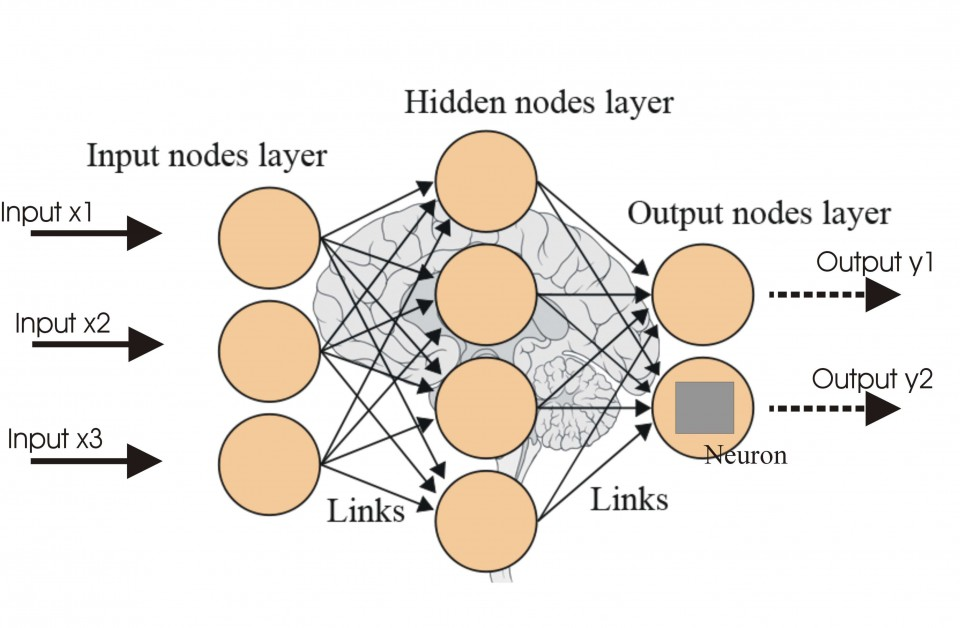
\includegraphics[width=0.5\linewidth]{images/principle.jpg}
\caption{Basic concept of a Neural Network}
\label{fig:principle}

\end{figure}

\end{frame}

\subsection{Background and Motivation - Convolutional Neural Networks}
\begin{frame}{Background and Motivation - Convolutional Neural Networks}
Convolutional Neural Networks (CNNs) are a subtype of Neural Networks:
  \begin{itemize}
     \item all neurons in a layer are identical 
     \item layers are interconnected through a kernel function
     \item different types of layers are used %(input, convolutional layer, RELU/tanh, maxpool,output
  \end{itemize}
\end{frame}
\begin{frame}{Background and Motivation - Convolutional Neural Networks}
\begin{figure}
\centering
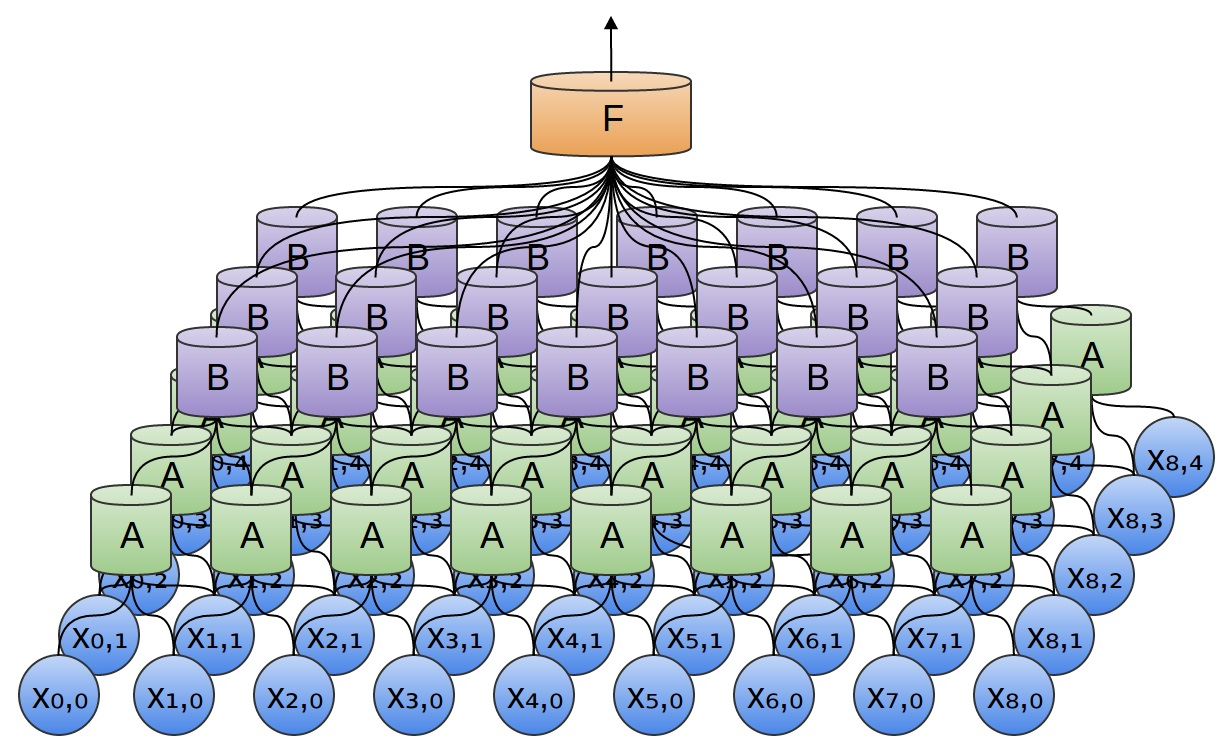
\includegraphics[width = 0.4\linewidth]{images/convexample.jpg}
\caption{2-dimensional CNN}
\label{fig:principle}
\end{figure}
\begin{enumerate}
\item Using identical copies of the same neuron allows for complex models with few parameters
\item Convolutional layers are not fully connected; each neurons is locally connected with a subsection of the previous layer
\end{enumerate}
\end{frame}
\begin{frame}{Background and Motivation - Convolutional Neural Networks}

\end{frame}
\section{Propagation}
\begin{frame}{Propagation - Forward Propagation}
Forward propagation is  the process of computing the output of a network for a given input
 \begin{figure}
\centering
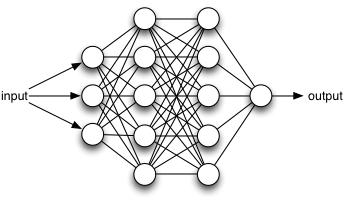
\includegraphics[width = 0.4\linewidth]{images/forwardpropagation.png}
\caption{Forward propagation in a complex neural network}

The 
\label{fig:principle}
\end{figure}
\end{frame}




\subsection{Kernel function}
\begin{frame}



\end{frame}
%\subsection{Layers}
%\begin{frame}{Layers - Input}
%\huge
%Inputlayer
%\newline
%\normalsize
%The input layer consists of an n-dimensional matrix, which contain the information to be processed
%
%\begin{itemize}
%\item Our example uses a 2-dimensional input which represents the pixels of the images
%\item asd
%\end{itemize}
%
%
%
%\end{frame}
%
%
%\begin{frame}{Layers - Convolution}
%The neurons of the Convolutional Layer is connected to the output of the previous layer through the kernel-function. 
%\end{frame}
%
%\begin{frame}{RELU/tanh layer}
%%The RELU layer (from rectified linear units) is a fully connected layer which implements the threshold function $y  = max(0,x)$. It adds non linearity to the network, which would otherwise be identical to a single layer perceptron. This makes the approximation of nonlinear functions possible. \newline Recent research has found a different activation function, the rectified linear function, often works better in practice for deep neural networks. This activation function is different from sigmoid and tanh http://ufldl.stanford.edu/tutorial/supervised/MultiLayerNeuralNetworks/
%
%because it is not bounded or continuously differentiable. The rectified linear activation function is given by,
%f(z)=max(0,x).
%
%To make backpropagation easier we used a differentiable function similar to RELU: $y = ln(1+e^x)$
%\end{frame}
%
%\begin{frame}{Max-Pooling layer}
%The Max-Pooling layer partitions the image, returns the maximum value of each partition   and returns a compressed version of the input. This is done to a) reduce overfitting and b) downsampling the input
%
%
%\end{frame}
%\begin{frame}{Dropout Layer}
%The dropout layer is a fully connected layer. It reduces overfitting and downsamples the input by randomly dropping neurons and their connections during training. 
%
%\end{frame}
%\begin{frame}{Dense layer}
%The dense layer is identical to a normal neural network layer in that it is fully interconnected with every neuron of the previous layer.
%\linebreak
%image here
%\end{frame}
%
%\begin{frame}{Output layer}
%The output layer is fully connected and unambigously assigns each neuron of the output to one of the expected results.
%\linebreak
%image here
%\end{frame}



\begin{thebibliography}{9}
\small
\bibitem{lamport94}
  Leslie Lamport,
  \emph{\LaTeX: a document preparation system},
  Addison Wesley, Massachusetts,
  2nd edition,
  1994.
@misc{bworld,
  author = {Christian Perone},
  title = {{Deep learning – Convolutional neural networks and feature extraction with Python}},
  howpublished = "\url{http://blog.christianperone.com/2015/08/convolutional-neural-networks-and-feature-extraction-with-python/}",
  year = {2015}, 
  note = "[Online; accessed 21.01.2017]"
}
%figures 1 and 2 from http://cs231n.github.io/neural-networks-1/#bio
%figure 3 http://futurehumanevolution.com/artificial-intelligence-future-human-evolution/artificial-neural-networks
% figure 4 http://colah.github.io/posts/2014-07-Conv-Nets-Modular/
% https://bfeba431-a-62cb3a1a-s-sites.googlegroups.com/site/deeplearningcvpr2014/ranzato_cvpr2014_DLtutorial.pdf?attachauth=ANoY7cpoT6OKao2g3iqQB4JqrLBF4e9GfZ06wOsnqfD_Dy5aob09rA3XzGPQSysUphYafHjkncEfoJPPyab19s4v8tfQS65Xk57NWieQOFC1zrYR2O_0gUN1Bsb64TS6kucrQP2prHjwwO4-Bc_9IRzGfWtlSMUGL_SxZnW_uSJHNbCzTQSfeZicjRxOCsBCNcA-4ifO2z8HaCqegyP8LQQGlp9gA7bPiIva1wxa69xKa7PB0iipEVWW180McZkDbBjefD0Thr13&attredirects=0
%figure forward propagation http://briandolhansky.com/blog/2013/9/27/artificial-neural-networks-backpropagation-part-4
% back propagation: http://neuralnetworksanddeeplearning.com/chap2.html
http://cs231n.github.io/convolutional-networks/
http://colah.github.io/posts/2014-07-Conv-Nets-Modular/
\end{thebibliography}
\end{document}